\chapter{You are your stories}
\addcontentsline{toc}{chapterdescription}{Your meaning-making stories generate your experienced reality from a limited slice of what actually is. Your stories lie in a self-consistent category, or stage of meaning-making; they form frames of reference that you use to evaluate and judge what is happening, giving it meaning. Using the Ground Pattern you can grow bigger meaning-making stories, so that you can rise to your adaptive challenges.}
%\addcontentsline{toc}{chapterdescription}{\pagebreak}
\label{chapter:who-am-i-meaning}


\begin{chapterquotation}
We all know that Art is not Truth. Art is a lie that makes us realise truth, at least the truth that is given us to understand. The artist must know the manner whereby to convince others of the truthfulness of his lies. \\
\raggedleft\textemdash Pablo Picasso\index{Picasso, Pablo}
\end{chapterquotation}


\section{Your stories make meaning}
We humans are the best at seeing patterns and giving meaning to them by applying one of our pre-existing meaning-making story \index{meaning-making stories} templates. We only start work on creating new meaning-making story templates, i.e., change our self, when none of our existing ones work for the adaptive challenge we are facing\footnote{This chapter was sponsored by Vet Dynamics UK}. 


Because it's so important, it's worth repeating: the reality you experience is created by the meaning making of your stories.


To experience a different reality\index{reality}, you need to change the stories you use to make meaning. Of course, there are very real and hard limits to what you can and cannot change. Simply telling yourself a story that denies climate change, or your height, does not alter the actuality of climate change, nor your height. However, what climate change or your height means to you is shaped by your stories, and you have the power to change these. If you want to do something, but believe that there is nothing you can do, first look at how you can change the stories that create your meaning, a reality you inhabit and are powerless in.


Figuring out how to change your meaning-making story used to be a trial and error, hit and miss process. Fortunately, the past few decades in adult development have shown clearly\cite{constantin-are-developmental-stages-real} that our meaning-making stories come in distinct categories, or stages, a progression of the clear stages of child development. Each category of stories builds on the foundation of the earlier categories, and forms the foundation of the later category. You can't skip a category. Hence, these categories are commonly called stages. 


If you know which category your current stories belong to, you can see more clearly which experiences you need to create for yourself so that you can grow your story templates towards the next category.


No stage is better or worse in absolute than another stage, just as classical physics\index{physics!classical} is neither better nor worse than quantum physics\index{physics!quantum}, even though they are sequential. Rather, like classical physics is best at describing what we can say about the world when things are relatively big, and quantum physics is best at describing the world of everything that is relatively small, the same is true of the stages of adult development\index{stages of adult development}. Each stage is best at some aspect of being human in human society, each is essential, and requires the previous stage as foundation. 


You grow yourself from one stage to the next by chipping away all parts of your old stories that are no longer helpful, and adding new stories that are more helpful in making viable, actionable meaning of the adaptive challenge you are facing. The best way to do this is by creating experiences that give your stories conflicting input so that they rewrite themselves.


There is no way for you to consciously rewrite your stories\index{stories}. The stories are you, they have written themselves up until now, and they will continue to write themselves. There is no way of saying to yourself, let alone to somebody else, \emph{“if you follow this 10-step plan, and work hard, you will get to the next stage in six months.”}


In fact, it's more like the joke about the disciple who asked his guru, 
\begin{quotation}
 “Master, how long will it take me to get enlightened?”
\emph{To which the master replied}, “probably about 10 to 15 years.”
 “And if I work really hard at it, how long then, guru?”
 “Oh, I imagine then it will be completely different. Then it will take you about 40 years.”
\end{quotation}


Each successive stage is a new paradigm of ever broader and more complex enlightenment. That means a broader and more comprehensive paradigm that sheds light on completely different ways of seeing yourself and others, with completely different yardsticks. 


Once you have learnt this new paradigm, you can never unlearn it.


What triggers each step in your journey is a growing awareness that how you describe what is, is not capable of handling what \emph{actually is}. And this creates the drive to break free from your current paradigms and shift into a more comprehensive paradigm, which includes everything still useful in the old paradigm, just as quantum mechanics\index{mechanics!quantum} still includes everything that is useful from classical mechanics\index{mechanics!classical}, and even becomes completely classical mechanics in certain situations. 


In the next chapter, you will see how to use a set of Adaptive Way\index{Adaptive Way} patterns that I have so far found to be the best at identifying what in my meaning-making story can change, and which experiences can lead it to rewrite itself. But first let's look at the Constructive Developmental Framework (CDF)\index{Constructive Developmental Framework} definition of the six stages of adult meaning making.
\subsection{Stages of meaning making}
\label{section:dev-stages}\index{meaning-making!six stages of|(}


The six stages are listed below and depicted in Figure~\ref{fig:social-emotional-stages}. 


\begin{description}
\item [S1: Impulsive mind.] Your immediate impulses occupy centre stage and drive you to act almost without any conscious thought. Most people move to the next stage while still children, or at the latest as teenagers. You're unlikely to meet somebody at work who still has their centre of gravity at S1.
\item [S2: Instrumental mind.] Your individual needs, and how to meet them, is the central theme of most of your stories. Over 10\% of the population remains at this stage throughout their adult life.
\item [S3: Socialised mind.] Your stories are primarily centred around what it means to be accepted and valued by other people. The stories now enable you to meet your needs through peer collaboration, whereas at S2 you're more likely to focus on meeting your needs directly or through power over another. Over 55\% of the population reaches and then remains at this stage.
\item [S4: Self-authoring mind.] Your stories are now centred on the values and unique concept of integrity that you have created for yourself independently of other people’s expectations. Approximately 25\% of people progress  this far. This is the first stage with the full developmental capacity to manage other people effectively (especially knowledge workers), or to fully use the potential of self-governing or self-organising approaches like Sociocracy\index{Sociocracy} or Holacracy.\index{Holacracy}
\item [S5: Self-aware and self-transforming.] You are now fully aware of all the different aspects of your self-constructed identity, see them all as valid and none as absolutely superior to any others. You are quite comfortable that some of your stories defining who you are are deeply incompatible with other stories of who you are. Your stories,\index{stories} and who you are, are now deeply fluid, enabling you to easily write the new stories that will turn you into whoever you need to be to address whichever new challenge comes your way. Less than 8\% progress to this stage.
\item [S6] Stage~6 and any stages beyond have yet to be sufficiently understood, and are beyond the scope of this book.
\end{description}




\begin{figure}[htb]
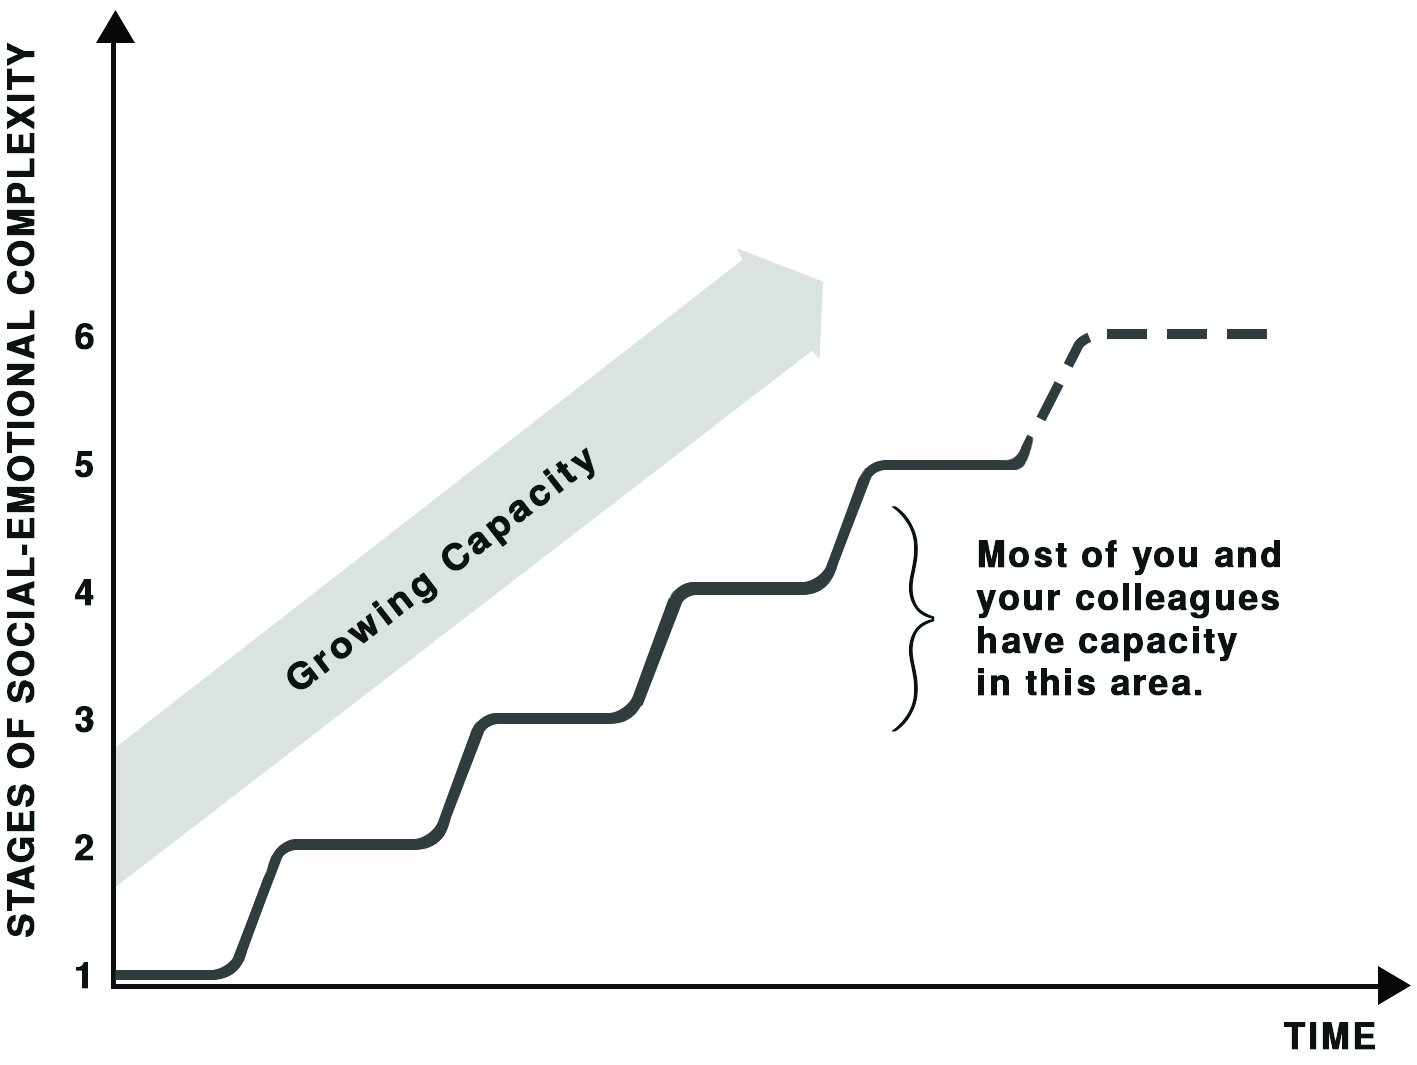
\includegraphics[width=0.95\textwidth]{./Images/Socio-Emo-Stages}
\caption[Social-emotional / meaning-making capacity]{Stages of social-emotional / meaning-making capacity growth. Most of you, and your colleagues, are likely to have a capacity in the bracketted range, from entering stage~3 to stable at stage~4. This diagram is derived from Kegan\index{Kegan, Robert} and Lahey\cite{kegan-immunity}.}\index{Lahey, Lisa}
\label{fig:social-emotional-stages}
\end{figure}


At work you will mostly find people at stages~3 and~4, with a few on their way from stage~2 to 3, or from stage~4 to~5. Very few will have their centre of gravity at stage~5, and even fewer at stage~6. In fact, stage~6 is not yet well understood; there are too few people at stage~6 to have a good enough idea of what it looks like.


Each stage has a clearly identifiable and self-consistent set of stories. 


I cannot emphasise enough: having your stories primarily centred on a specific stage does not make you a better person than someone whose stories are centred at any of the others. You will not necessarily be any happier if you are at a different stage to the one you are in now, nor any wealthier. Every society and organisation needs people at all stages, and every stage is essential to meet all challenges. 


And remember, the stage is only about your stories; each stage has a wide range of different personalities, different fluidity in the different types of thinking, different hardwired needs, different values and ideals. Useful as it is in making it easier for you to rewrite your stories, never forget that you cannot actually separate your stories from everything else about you. You are one integrated whole, the structures of your thinking, the patterns of your meaning-making stories, all their content, along with your physical body. 


Some in positions of influence today are between S3 and S4. Someone who is here has typically differentiated themselves towards becoming unique, but still derives some of their self-identity through belonging to a self-selecting group of people who are similarly different to the general population. In some cases, this is through belonging to a community of expert practitioners in some discipline.


Then you have someone who defines their worth, their self-identity, and who anchors their meaning-making stories in other people seeing them as an expert. There is a huge difference between somebody who is at S4 or beyond and \emph{has} expertise and somebody who has not yet reached S4 who's meaning-making story says \begin{quote} I \emph{am} an expert. \end{quote} 


This expert stage encompasses those who are unable to differentiate between \emph{having} expertise versus \emph{being} an expert. They can easily become a barrier to progress because any challenge to their discipline is interpreted as a challenge to their worthiness as a human being\textemdash a life-threatening challenge because if you take away the validity of their expertise, it's tantamount to the death of their identity.


All disciplines have this. Expert-stage climate scientists are a barrier to public understanding of the climate emergency; expert-stage economists are a barrier to the adoption of more useful models of our economy; expert-stage lawyers are a barrier to reinventing company law, and so on across all disciplines. (My (Graham) \emph{being} an expert has at times been a barrier to achieving my goals.)


There is a world of difference between people who have expertise (we need many more of these) and people who derive their identity, the validity of their being, from being identified by themselves and others as being an expert.


We have a higher need than ever before for people who have progressed through the expert intermediate stage, retaining all their expertise but no longer identifying themselves with belonging to their discipline. This begins with S4, and then S5, as stages that have an identity, or meaning-making stories, independent of others’ expectations. 


From S4 onwards you become capable of leading management hierarchies effectively, of leading major change programmes, and in particular leading the change from a traditional organisational hierarchy to a self-governing developmental organisation. From S4 onwards you are adept at working with people from very different disciplines to yours, including those whose discipline contradicts some of your tenets. 


But we have fewer people at S4 than we need, and even fewer at S5. 


We need more at these stages than ever before because we now have so many large organisations needing significant numbers of people managers and leaders of system transformation. Less than 33\% of the adult population ever progresses to these stages, often only towards the end of their working lives, or after retirement. Our current concept of retirement, and age-segregated living, has lost us many of the benefits we need.


Most of the frames of reference\index{frames of reference} that your stories\index{stories} give you are so obvious to you, and so deep inside you, that you can no longer see them. You are unaware that they are there. The ground pattern of Section~\ref{section:ground-pattern} is the best method we have found of sneaking up on your hidden stories and shining a spotlight on them faster than they can run away and hide. Then you can create the optimum experiences for your stories to adapt themselves, and for you to move to the next stage. Feel free to go straight to Section~\ref{section:ground-pattern} if you want to start now.


But no one can just read up on a new stage of meaning making and quickly adopt it. You have to construct it through experiences and reflection. You can, however, learn new forms of thought quite rapidly. We cover the 28 transformational forms of thought in Chapter~\ref{chapter:who-am-i-sense}. The more fluidity you have in them, the easier it will be for you to create powerful experiences you need for your stories to rewrite themselves. 


Here's an example from one of my clients to illustrate how one of these stages shows up in the workplace, for two people I will call Cathy and Janet\footnote{Not their real names.}. 


\begin{longstoryblock}
Cathy and Janet both work for the same company and have the same specialisation. Janet is new and on a steep learning curve about how to work in her speciality, and how to work with colleagues. Cathy is new in the role of being the leader of a colleague and is breaking free of her old big assumptions around taking care of people. 


Almost everything Janet does is for the first time. She acts from a frame of reference that says that any sensible person will look to their managers, and anyone with more experience, for guidance on what is expected. Also, any sensible person will also observe closely what more experienced people are doing, interpret that as the way to succeed around here, and mimic them. (Or, as the way to fail around here, and so do the opposite!)


Janet imitates what others are doing, how they behave, dress etc. 


Cathy has a very different set of stories to Janet. Some of Cathy's are about independence and avoiding being overloaded by trying to take care of too many other people’s needs. 


So when Janet is imitating Cathy, or asking Cathy questions, Cathy makes the meaning: \emph{Janet is asking me to take care of her.} Because Cathy is rebelling subconsciously against these old meaning-making scripts imposed on her by her parents, her hidden commitments kick in, and she, misinterpreting the meaning in Janet's words and actions, tells Janet to get lost.


Cathy is beginning to attempt, in a clumsy way, to define her identity independently of belonging to any group by simply adopting the group norms of behaviour and identity.


Janet then makes meaning of Cathy's actions as \emph{ Cathy is a cold, demanding, uncaring woman. I need to fix the problems she is causing.} By helping Cathy to bond with the group by conforming to its behavioural norms. 


Now we have a perfect spiral of mismatched meaning making, leading inexorably to a dysfunctional working relationship, even though each is doing the very best they can to collaborate.
\end{longstoryblock}


The most commonly found stage in any organisation is S3, or the socialised mind. This is the stage that society needs most people to be at for society to be stable. It is the central stage that reflects one of our superpowers: the power to live and work together in groups by adopting the common stories as your own. 


On the other hand, Stages~2 and~4 are both quite individualistic, so it costs the group far more effort to maintain social bonding of members at Stage~2 or~4 than at Stage~3. 


Any healthy group that thrives long term through many major challenges requires enough people at each stage and a way of working with people at different stages. This is a big challenge for companies today.\index{meaning-making!six stages of|)}


\subsection{Judgements and frames of reference} 
You cannot \emph{not} make judgements. Trying to become someone who is non\hyp{}judgemental is inherently impossible because the reality you experience is created by the judgements hidden deep in your stories, and that you are therefore subject to.


The best you can do is hold your judgements lightly, as information, not blindly following them.


Your stories are the frames of reference\index{frames of reference}, you use to generate judgements in your reality. 


Instead of striving for the impossible goal of becoming free of judgement (because making meaning is evaluating and judging), put your effort into becoming aware of your stories, and how they shape the reality that you experience. Like the film projector analogy, the more you understand how the light, film, lens, and screen all shape the reality you experience, the more able you are to experience with your full potential everything that actually is.


The more you can shift your stories from hidden ones that you are subject to into conscious ones, the more able you are to recognise when one of your stories is past its sell-by date, a frame of reference holding you back. When it is necessary to pull out a different story from your library and use that as a valid frame of reference, or even when it's time to adapt yourself to rise to a challenge you've never experienced before by writing a brand new story.


I sometimes used to judge colleagues as incompetent idiots if they didn't see things my way. Not any more (or at least, not for more than a few minutes) because I now manage to remind myself quickly that the judgement is coming from my frame of reference. It is giving meaning to only the small part that I take in of everything that is happening. Then I can work out if the issue is actuality\textemdash the person truly is an incompetent idiot\textemdash or my inner reality, shaped and given meaning by my stories. Usually it is a mixture of both!


In the story of Cathy and Janet above, neither sees the whole, unbiased actuality. Each can only work off their own experience of their reality, shaped by their own stories. Each shapes the unique realities they each experience, including the underlying intention they project onto the other. So the “why” that Cathy attributes to Janet's behaviour is not Janet's why. It is, if Cathy ever did what Janet has done, the reason why Cathy would do that. Which has nothing to do with Janet.


Your judgement about why you think someone does what they do comes from your own frame of reference. You may be completely right, you may be partially right, or you may be completely wrong. But either way, keep a very close eye on yourself. Explore how you may be misinterpreting why someone else is doing something. Mis-interpreting because you are looking at them and their actions through the distorting lenses of your own meaning making.


This might be a good time to reflect on where the judgements of Picasso\index{Picasso, Pablo} and Einstein\index{Einstein, Albert} came from, both positive and negative, referred to in Section~\ref{section:intro-your-ad-cap}. 


\subsection{Winning and losing}
Beauty is in the eye of the beholder. Marmalade-coloured cats, never hippos, win my animal beauty pageant. But that hippo’s mum thinks her baby hippo is the most beautiful being ever. 


Nature disagrees with both of us; nature sees cats and hippos as each just right for their niche in the ecosystem, each as vital, integral parts of life on the planet. Nature uses a completely different frame of reference.


Success and failure are also in the eye of the beholder. 


\begin{longstoryblock}
There are those who see me as a failure, because 12 years ago I (Graham) stepped away from a rapidly advancing career with Procter and Gamble\index{Procter and Gamble} to focus on using the power of business to combat our climate crisis. Others see me as a success for precisely the same reason.


In the shower this morning I started to judge myself as a failure because I was looking at what I have achieved over the past 12 years. And then I caught myself and remembered that, just a week ago, I’d judged myself a huge success, because I'd inspired and moved people I admired, at a conference in Tuscany. People saw that I have developed, with the Adaptive Organisation that includes the FairShares Commons\index{FairShares Commons} described in this book, the foundations for a fundamentally new way of doing business. One that is the foundation for combatting climate change without creating even more problems.


I quickly came back into balance, as I became aware of the bigger picture. Firstly, in each case, my judgement was based on a small fraction of everything that I have achieved over the past 12 years. Most of what I have achieved I cannot know about because it lies in what other people have become and done because of how I have triggered movement in them. Secondly, every time I judge myself, or anyone else, I can only do so by comparing what I see to my own unique internal yardstick.


\begin{enumerate}
\item What I see depends on which lens(es)\index{lens} I choose to use, out of the infinitely many lenses I could use. Each lens shows a part of what actually is, with some kind of distortion, but none can possibly show all that actually is without any distortion. Every time you judge yourself as a success, or as a failure, check which lens you are using to look at the data. Then ask yourself, which data is completely hidden by that lens, and which data is distorted by that lens?
\item How I then judge what I see, a distorted fraction of what is, depends on which of my many self-constructed yardsticks I choose to use (Chapter~\ref{chapter:who-am-i-sense}, P5 and C6). Every time you judge yourself as a success, or as a failure, check which yardstick you are using. How do you know that that yardstick is at all relevant? If it is relevant, are there other yardsticks that may be equally relevant, and that you also ought to use, because they point to a different judgement? What are all the yardsticks that you need to use simultaneously to minimise the risk of self-deception? (Even if some of them contradict each other.)
\end{enumerate}


\end{longstoryblock}


There is no absolute success, nor absolute failure, in any part of life, and certainly not as a startup founder, manager or leader. You have succeeded, simply by being born and continuing to breathe until the breath of life leaves you again. At least, I believe that that is how nature defines success for any living being. 


Success and failure lie purely in the lenses and frames of reference\index{frames of reference} you are able to use, and in whether or not you give these lenses and frames of reference any validity. Which depends on your stories, and how strongly you believe in them.


I’m getting better at using whatever happens as information about whether


\begin{enumerate}
\item what I’m doing is more or less helpful to achieving my goals;
\item or my goals are illusions created by the distortions of my lenses and frames of reference;
\item and not as triggers for feeling hope or despair because I judge myself as a success or a failure.
\end{enumerate}


For example, I came out of the shower this morning feeling relaxed, seeing both success and failure as an inseparable part of what I am doing, which left me calm and energised to continue writing this book. 


Judging yourself as a success or as a failure is one of the most common judgements we make about ourselves. Often this judgement is at best incomplete, and at worst totally false. Judging yourself as either a success or as a failure can be the self-deception that enables you to succeed; or that prevents you from succeeding. 


Three related topics that hold many potential entrepreneurs back from the results they could achieve lie in their relationship with money\cite{dellner-money, twist-money}\index{Twist, Lynne},  power\cite{kahane-power-and-love}, and imposter syndrome. These are common challenges for many, and can be very effectively transformed by working on the meaning-making stories that create them via the Adaptive Way Ground Pattern in the next section.
\section{Grow better, bigger stories}
\label{section:ground-pattern}


\begin{quotation}
Faced with the choice between changing one's mind and proving that there is no need to do so, almost everyone gets busy on the proof. \\
\raggedleft\textemdash John Kenneth Galbraith\cite{galbraith-mind}\index{Galbraith, John Kenneth}
\end{quotation}


In this section you will read an abbreviated version of the Evolutesix Adaptive Way ground pattern (GP)\footnote{
The sources of inspiration for the Evolutesix Adaptive Way ground pattern include Robert Kegan\index{Kegan, Robert} and Lisa Lahey\index{Lahey, Lisa}, \emph{Immunity to Change}\cite{kegan-immunity}\index{Immunity to Change} and \emph{How The Way we Talk Can Change The Way We Work}\cite{kegan-talk}; \index{How The Way we Talk Can Change The Way We Work} the non-violent communication (NVC) of Marshall Rosenberg\cite{rosenberg-nvc};\index{Rosenberg, Marshall} Byron Katie's \emph{The Work}\cite{katie-work}; \index{Katie, Byron}and \emph{Big Heart Big Mind} by Genpo Roshi\cite{roshi-big}.\index{Roshi, Genpo} 


The research described by Timothy Wilson\index{Wilson, Timothy} in \emph{Redirect}\cite{wilson-redirect}, Steve Salerno\index{Salerno, Steve} in \emph{SHAM}\cite{salerno-sham} and Miguel Farias\index{Farias, Miguel} in \emph{The Buddha Pill: Can Meditation Change You?}\cite{farias-buddha}\index{The Buddha Pill} on how ineffective, or even harmful, many of the approaches to behavioural change and self-help are, have guided what I include in the Adaptive Way.\index{Adaptive Way}
}, which is covered in far more detail in my (Graham’s) forthcoming books\cite{boyd-regenerate}. 


The ground pattern is a sophisticated dialogue tool, both for your inner dialogue, and for dialogue with others, to recognise and transform meaning-making stories.\index{meaning-making stories} 


Once you have constructed a newer map that is more realistic and more useful, you will be able to get more helpful answers to your questions \emph{“How am I? Who am I? Who should I do what for? Who can I become as I grow up, and what will help me change, so that I become that next version of me?”} 


The Evolutesix Adaptive Way’s\index{Adaptive Way} big advantage lies in the clarity it gives you, because the strict use of patterns separates and so clarifies the often messy mix of all your different goals, activities, feelings, judgements, beliefs, and nature. I (Graham) have found this magical, for myself, and even more so working with others. 


Many approaches to developing yourself begin with complaints, as the ground pattern does, but instead then exhort you to declare yourself to just be different or do differently, without providing any viable way of changing the underlying meaning-making stories that are who you are and that create the reality you experience. So they fail, at best; and at worst, are contributing to the growing rise of depression and other psychological issues\cite{wilson-redirect}. 


The ground pattern works because it takes into account you as a full living being, keeping all aspects of what makes you who you are and that shape the reality you experience.


Please hold tightly to the strictness of the pattern at first. Only once you are really fluid at using it strictly are you likely to be able to use it in an improvised jazz fashion, without misinterpreting what the conflict you are experiencing is actually telling you about how to adapt yourself.


\subsubsection[GP Step~1: From Complaints to Aspirational Commitments] {GP Step~1: Goals,\index{ground pattern|(} 
or translating from Complaints to Aspirational Commitments.}
\textbf{Purpose: Identify your goal(s), or what is important or valuable to you, even better, your underlying needs. We call this an aspirational commitment.} ~


The endpoint of this GP step is having a clear commitment sentence:


\begin{quote}
I am actively committed to (achieving / the value of / the importance of / the need
\footnote{Need\index{needs} in this book usually means need in the way Marshall Rosenberg\index{Rosenberg, Marshall} defines it in his non-violent communication. See the list of the more common needs in tables~\ref{table:needs-top} and~\ref{table:needs-all}. The important distinction between needs in an NVC or our ground pattern and common speech is that here a need is yours, inside you, and not linked to any other person. For example, any time anyone says to you “I need you to …”, that is not a need. You are not their need. They have a need, perhaps a need for safety, and they are choosing you as a tool to meet that need. Beware of being coerced into becoming their tool. Master these dojo patterns to recognise such coercion. It is very common in how we learn to talk to each other these days!} 
for) \ldots
\end{quote}


You might already have commitments clearly defined, as a clear goal. Some objective or achievement you have already set your sights on. Perhaps the next promotion, getting a pay rise, or whatever. Then finding these commitments is easy. 


You also have commitments that are not yet sufficiently clearly defined. So long as there is anything where you are complaining about what is not, rather than talking about what you want that is valuable or important to you, you can benefit from getting more clarity on your commitment by mining them out of your complaints. 


Unlike what many managers think, complaints are valuable. Encouraging complaints in order to mine the value in them gives you what you need to develop. Look at complaints as the best that you can do, within your current reality, to communicate to yourself and the people around you that something is not sufficiently fit for purpose. The worst thing that anyone, let alone someone leading a process, can do, is to shut down your talking about what you can feel but cannot yet articulate. Feelings are hard data that cannot be put into rational words. 


If you are in a meeting, for example, work on any feelings and complaints until you are clear whether or not they are telling you something you must take into account to have any hope of achieving the purpose of that meeting. I (Graham) certainly wish I had been able to do this far better ten years ago in P\&G.
 
Any complaints people have can be translated into an underlying unmet commitment, or need. Start by connecting with your emotions. Most likely you will come up with a number of commitments. Work with one at a time, and start a new ground pattern for each commitment.


To get your commitment into the clearest and most actionable strictness, complete the commitment sentence stem:


\begin{quote}
Therefore I am committed to the goal / value of / importance of / need for \ldots .
\end{quote}


Keep your aspirational commitments simple and actionable. Avoid any temptation you may have towards perfection, going ever deeper into abstract commitments, or in integrating multiple commitments into one more abstract commitment. You can easily get caught up in the joy of getting ever deeper insights into your deepest, clearest needs (summarised in the tables of Section~\ref{section:needs}), and remain at the commitment GP step. 


If you find yourself staying at GP step~1 in a search for deeper insight and perfection, check if this search for insight and perfection is one of your blocking behaviours of the next GP step. If so, your hidden commitments (GP step~3) have kicked in, and you are protecting one of your vulnerabilities in thinking you cannot move forwards until you have found the deepest, purest commitment. 


Keep it simple, approach it playfully with an improv mindset, and move forwards fast, but imperfectly. Be a playful entrepreneur or leader\cite{dodgson-playful-entrepreneur}!


Sometimes it feels clumsy to use the full sentence stem. Instead you might want to say, for example, \emph{I'm committed to building my website} or \emph{building my website is important to me.} Sometimes that form is the best way to go. If it works for you, use it. Just keep in mind, especially at the beginning, when you are coaching yourself, mediating between the different voices in your head, using the pure structure prevents you from getting lost in your own circles. It keeps you moving forwards.


Using the words \emph{value of} or \emph{importance of} or \emph{need for} brings three things into sharp clarity:


\begin{enumerate}
\item Is it really important or valuable to you? Or is this just something that you have had put on your shoulders?
\item Is there something deeper? The sentence stems \emph{value / importance of / need for} are especially useful when wrestling with a fuzzy set of complaints. They help clarify the underlying needs or values that are poorly met in what you are doing. By stating them clearly then you can go on to identify in the next step why they are not met.
\item Is this expressed clearly as something universal, or at least something that many people will share with you? For example, \emph{I'm committed to being honest} is about you. \emph{I'm committed to the importance of / need for honesty} applies to you and everyone else. This lets you recognise why you have some complaints about others, but instead of trying to fix them, you can now focus on what is in your power to change. You can then explore in GP Step~2 the things you are doing that blocks other people from being honest with you as well. How you are (perhaps unintentionally) demanding that they lie to you.
\end{enumerate}


\subsubsection{GP Step~2: From self-blame and shame to self-compassion}


\paragraph{Purpose: Begin to transform yourself, by changing your perception of yourself from one of weakness, shame, and blame for your bad behaviours, to one of self-compassion, accepting that you are doing what you do for some good reason.} ~


Attempting to just change your behaviour never works. So long as the reason (usually a good reason, at least within your inner reality.) behind the behaviour remains, you will continue to block yourself from achieving your goals. Maybe with the same behaviour (and then you will feel even worse, and judge yourself even weaker) or with an alternate behaviour. Likely an even more extreme one. 


So in this section we begin the journey of mapping yourself, by sneaking up on that reason from behind, so that it does not hide away as it usually does. You will begin by identifying all the behaviours that hold you back from fulfilling the aspirational commitment identified in GP step~1 above. Both what you are doing that holds you back, as well as what you should be doing, but are not doing, and by neglecting to do, you are holding yourself back. 


By the end you will have a list of enough of these blocking behaviours to move on to GP step~3, the hidden commitment, as well as clarity on how you feel when you do these blocking behaviours, and how you judge yourself for doing them.


The intention in GP step~2 is to plant seeds for actionable hope by exploring yourself. You will have more clarity on what you are doing to block your aspirational commitments, and why. You will have learnt how to explore yourself by using the hard data in your feelings, and judgements about yourself. Data telling you about the underlying script you use to attribute meaning. 


You will be able to accept without judgement, instead with self-compassion, the simple fact that you are doing these blocking behaviours for good reasons. Recognising, though, that some of these reasons, whilst essential and valid in another context (e.g., as a five-year-old) are no longer essential as a 55-year-old!


If you are like almost everyone else, you are doing a number of things that hold you back from achieving your goals. In some ways, you are sabotaging yourself. GP step~2 will help you, and you can help your sparring partner, become aware of what works against your goals, or aspirational commitments. 


The objective here is to collect sufficient information for GP step~3, not to compile an exhaustive list of all blocking behaviours. You may find that this list is already partly there, in the complaints you used to identify your aspirational commitments.


If you primarily complained about the behaviour of others, now is the time to look for which of your behaviours might be contributing in some way to blocking you from achieving your aspirational commitment. You may well be the victim of other people’s behaviour, out of your control; but there is often something you are doing that contributes to holding you back from achieving your aspirational commitment. Something that is in your control. 


All you ever can work on is what is in your control, even if it is only 0.1\% of what creates the situation.


This is even more important if your aspirational commitment is on the edge of your circle of influence, like being committed to the importance of leaving behind you a healthy planet for the next generations to live on. For an aspirational commitment like this, the ground pattern is powerful, provided you focus on the fraction of a percent that you own. 


Only your words, actions and thoughts can ever be inside your circle of control. 


Your focus is on what your behaviour contributes towards your aspirational commitment being satisfied, or that works against that process. Later you will master the different thinking patterns (Chapter~\ref{chapter:who-am-i-sense}), especially the transformational ones. The more you master these thinking patterns, the more effective you will be in working on aspirational commitments way outside your circle of control.


Here is the task for GP step~2, blocking behaviours. List as many examples as you need of the following two types of behaviours blocking you from achieving the aspirational commitment you chose in GP step~1 to work on. 


\begin{description}
\item[Doing.] Blocking through action. What do you do, but should not be doing, because it holds you back from fulfilling your aspirational commitment?
\item[Not Doing.] Blocking through inaction. What are the things I should be doing to fulfill my aspirational commitment, but I am not doing?
\end{description}


Now you are ready for the task of translating this into a language of personal responsibility. 


Look at all the judgements of blame, shame etc. and ask yourself \emph{how would I evaluate myself if I knew that I was doing these for a reason my subconscious believes is good, but perhaps is a reason that is no longer valid, or at least not valid in this specific situation?}


At the very least, suspend judgement of yourself for now, and shift your attitude to one of acceptance and personal responsibility. A language of blame can only get you to dysfunctional New Year's resolutions, as we will see next.


Even if others are 99.999\% responsible for what is happening, you still usually have something you are doing that you could change. Differentiate between the part that is in circumstances you cannot control, vs. the part where you do own responsibility. You cannot change something that is a law of physics, or inside the control of another.


So now you have this list of some of your behaviours holding you back from having your aspirational commitments fully realised. Everything you are doing and not doing. Make sure that these are observable, actual, factual behaviours, not judgements or interpretations coming out of your meaning-making stories. Then


\begin{quote}
Leave the behaviours alone! \\
Do \emph{not} try to change or fix anything! 
\end{quote}


The worst thing you can do is try to change behaviours directly, or to fix anything as if it were a problem to fix. Many other approaches do attempt to change these. Often via a resolution to change, i.e., a new year's resolution! 


Such attempts to change, or fix these blocking behaviours, can easily cause you long-lasting harm because they fail to take into account what the behaviours in your list are good for. They fail to take into account the situations where these very "blocking" behaviours are vital to protect you from harm. They fail to take into account what you actually still need them for!


Even if there is nothing you need them for any more, if your subconscious guardian angel still believes you need them, it will do everything possible to protect you by retaining them. In the next GP step you will learn what works when resolutions and fixes fail.




\subsubsection[GP step~3: Resolutions to hidden commitments]{GP step~3: Resolutions to hidden commitments}


\textbf{Purpose: identify which hidden commitments are at the core of your blocking behaviours, because they are actually there to protect you from perceived harm. Shift from a blame, shame-driven paradigm of resolutions (declarations that tomorrow you will be a different person) to a compassion driven paradigm of exploring your vulnerabilities.} ~


Hidden commitments are what you are committed to avoid or prevent from happening. They are subconscious. They are deeply hidden in the lessons you have learnt about what certain situations or events mean for you and other people; in other words, in the scripts you have constructed throughout your life to generate meaning from meaningless actual facts. 


If you are used to Richard Barrett's\index{Barrett, Richard} approach to values\cite{barrett-values}, these are limiting values; or, if you are familiar with NVC, you can think of these as when you are subconsciously meeting needs related to preventing harm.


Here is an example from when I (Graham) learnt rock climbing on Table Mountain in Cape Town a few decades ago.
\begin{longstoryblock}
I used to climb on Table Mountain\index{South Africa!Table Mountain}. I often felt fear when looking down the vertical rock face, even though I knew it was an easy climb, and I was roped in. Every time I began abseiling, I felt fear. 


Feeling that fear is perfectly justified. After all, without the rope, letting go of the mountain means a 500m vertical drop onto solid rock, and certain death. Or, if I'm unlucky, living maimed. So the very last thing I should do is anything attempting to simply make a resolution to not feel fear, or to bully myself to just do it. 


That would rob me of exactly what I need to protect myself from falling in another situation where I lacked a rope. It would rob me of the instinct to protect myself  going down an open staircase.


What I needed, and did, was a slow process of re-educating my automatic responses in the specific situation while rock-climbing.


I've not climbed for 20 years now, and my healthy fear of falling off cliffs is still with me, thankfully! Of course, it now kicks in again even if I am safely roped up. 
\end{longstoryblock}


Alex Honnold\cite{honnold-el-cap},\index{Honnold, Alex} the first person to do a solo unprotected free climb of El Capitan in Yosemite, took over two years to prepare for it. He attempted the climb once before his successful climb and realised very quickly into the climb that his meaning-making stories at that point were not where they needed to be. He immediately aborted the climb. He did not try to push through, or blame himself for being who he was at that moment. All our lives we are doing daily the equivalent to a solo unprotected climb. Trying to simply push against who you are is only going to get yourself hurt, and lead to far poorer results in your startup than you could otherwise achieve.


The hidden commitment is a commitment to avoid or prevent something we believe may harm us. It may be as obvious and natural as avoiding situations where we might fall off a cliff. Or as subtle as avoiding situations where we might be praised. 


Your hidden commitments have some value, and should never be just violently squashed. 
This is why declarations to simply change your behaviour usually fail, and can even be harmful to you. Most resolutions to simply stop doing something you have decided is a bad habit fail because they neglect all the situations where that habit is good.


This dysfunctionality of most approaches keeps many in the self-help industry rich: the approaches fail you in a way that leads you to come back for another.


So until we have explored ourselves thoroughly, understood exactly how we generate the meaning we see in neutral, meaningless actual facts, any declaration along the lines of \emph{as of now I resolve to be different} may well cause harm. 


In this GP step we are after your hidden commitment. If your aspirational commitment is your idea of heaven (if my aspirational commitment were always satisfied, my life would be heaven), your hidden commitment is your idea of hell. If this was always in your life, you would be miserable, and seriously at threat of harm and pain. Your hidden commitment is expressed by completing the sentence stem: 


\begin{quote} 
I am committed / work hard to avoid / prevent \ldots 
\end{quote}




To find out what it is they are protecting you from, we need to go through the same door they use to get you to do your blocking behaviours. Worry or fear. 
\paragraph{Worry Box}
Filling in your worry box\index{worry box} opens the door to seeing your hidden commitment clearly. In your worry box you fill in all the bad things you fear might happen if you failed to do your blocking behaviours.


To get at your worry box, take each behaviour in your list of blocking behaviours\index{blocking behaviour}, and imagine yourself doing the extreme opposite behaviour. 


The pattern here is:
\begin{quote} 
Imagine you are doing the extreme opposite behaviour to your blocking behaviour. Really picture it in your head. Take your time to do so and feel inside you. How does it make you feel? If you feel worry, fear or similar, what are the thoughts that cause you to worry?
\end{quote}


For example, a common blocking behaviour is keeping silent in meetings until everyone else has spoken, and so sometimes losing completely the opportunity to contribute because someone else has made your point. Now imagine doing the extreme opposite behaviour; immediately you have a thought, blurt it out.


Or perhaps you are one of those whose blocking behaviour is constantly blurting things out immediately, and wish you could keep your mouth shut until after you've thought a bit more, because you keep shooting yourself in the foot with what you say! Now imagine doing the extreme opposite behaviour, keeping your mouth shut until you have really thought it through. 


What are the thoughts of worry that go through your head as you picture yourself doing the extreme opposite behaviour? What do you imagine might go wrong? What do you feel as you imagine that? 


If your worry sounds like a respectable thing to be worried about (e.g., I worry that my team will be stressed) then you're off-track. If you can be proud to tell others that this is your worry, you are off-track. Remember, this GP step is about finding out what your personal idea of hell is. A sure signal you have found part of your hell is if you feel fear, and feel shame when you tell others about it. 


To support you in this, remember, you are here to explore and understand the hidden commitment, not fix it. Certainly not to judge it, but rather to have compassion for the very valid history you have, that made this hidden commitment vital to protect you. 


To go from your worry box to your hidden commitment, start by looking for any common themes across a few or even all of your worry box\index{worry box} entries. The hidden commitment lies where the largest discomfort is. Then complete the sentence stem:
 
\begin{quote}
I am (committed / work hard) to (avoid / prevent) \ldots .
\end{quote}


Get the sentence as concrete and specific as possible, e.g. 


\begin{quote} 
I am committed to preventing any situation where I am seen by others as not smart enough. \\ \emph{ Or } \\
I am committed to preventing any situation where I start to feel depressed. 
\end{quote}


Note that it is perfectly fine to have a hidden commitment to avoid some kind of feeling. We have found it quite common for certain types of feelings, like feeling depressed, overwhelmed, or lonely, to take on a life of their own. And once certain feelings do, merely having that feeling can become the primary threat to you. 


For example, I know that once I start to feel depressed, I can very easily get locked into a downward spiral. So preventing this spiral from starting becomes important for my productivity and happiness.


Hopefully you now realise that the image of an internal dialogue\index{dialogue} between your inner angel and devil is false. All that is actually happening is that you are pulling against yourself, because both your inner angel and your inner devil come out of the same set of meaning-making stories, unique to you. Your aspirational commitments and hidden commitments are like opposing teams in a football match, or in a tug of war, but you are both teams. In any war against yourself, there can only be one loser and no winner.


Part of what makes this a viable map of yourself is, as with any map, putting elements into the map in the same position that they are in the landscape. Recognising when a commitment belongs in GP step~1 or in GP step~3 is an art that is essential, and takes practice with a more experienced sparring partner to develop. Be careful not to confuse the complaints leading to an aspirational commitment of GP step~1 with the resolution to the hidden commitment of GP step~3. 


Also keep an eye open for situations where you have two or more aspirational commitments that cannot be simultaneously satisfied with one action. For example, I have a commitment to health, including a good night's sleep each night, and a commitment to excellence. Sometimes I have to choose which aspirational commitment I satisfy. This is quite different to the tension between aspirational and hidden commitments.


The relationship between the aspirational commitment and the hidden commitment is in your behaviour: you intend to fulfil your aspirational commitment, but your actual actions (by which you sabotage your aspirational commitment) follow a well-perfected strategy to fulfil your hidden commitment. To protect you from the harm in your personal hell.


\subsubsection{GP step~4: Big Assumptions}
\label{chapter:big-assumptions}


\textbf{Purpose: identify the big assumptions\index{assumptions} behind the hidden commitments, and that are a subcategory of the meaning-making stories that drive your choices and behaviours.} ~


A “big assumption” is what your meaning\hyp{}making tells you will happen if you fail to protect the vulnerability that your hidden commitment is committed to protecting. The big assumption is based on past lessons drawn from past experiences which might not apply to you today. Or perhaps only apply in certain specialised situations.


All your big assumptions, along with the stories that still drive you but you are now aware of, are the entire set of meaning-making stories that you use to construct your internal reality out of the inherently neutral facts you take in.


For example, one specialised situation where some of my big assumptions still apply is with my parents. In some ways, neither they nor I have quite accepted that I am now 50, not 15. 


The big assumption in the strict form that we use in the Adaptive Way\index{Adaptive Way} consists of four parts. 


\begin{enumerate}
\item If I fail to (\ldots my hidden commitment \ldots)
\item The emotional consequence of failing to fulfill your hidden commitment
\item The meaning you give to failing to fulfill your hidden commitment, and / or the meaning you give to the emotional consequences
\item The chain of consequences through to the worst-case end-point.
\end{enumerate}


Using the strict form at the start of your practice will make it easy to use this at work to collaborate effectively, to support each other in peer-to-peer sparring, and even more so to support yourself when using the pattern alone.


You might think, when you say or write down your big assumption, that it is clearly ridiculous. This is very common, and is a first loosening of the hold it has on you. But avoid going too fast, avoid falling into the trap of trying to fix your big assumption there and then. The big assumption is not a thing to be fixed, but rather a mystery to explore and transform into a more mature, wiser and useful meaning making script. One relevant to you now, rather than you way back then.


This is of vital importance. Most big assumptions have some element of usefulness in them. You want to preserve this usefulness at all costs, because it may well be a life-saver. You may have a big assumption saying \emph{If I fail to avoid angering people, I will feel scared and powerless, because it means I will be bullied and hurt, and then I'll be killed.} In some situations this big assumption is realistic and helps you deal effectively with, say, being taken hostage in an armed robbery.


Instead of trying to fix yourself, as if this big assumption is only and always a problem, but never a help to you, approach it from an appreciative stance\cite{cooperrider-ai}. In the more advanced Adaptive Way \index{Adaptive Way} patterns we develop your capacity to use appreciative inquiry as a basis for engaging with yourself, others, and the work of your organisation.


Look at all aspects of this big assumption and yourself. Treat yourself, and everything in your life, as a curriculum to learn from. The five steps in the transformational experiments part of the ground pattern, and the castle move, will support you even more in doing that.


You will often use this ground pattern in dialogue\index{dialogue} with your colleagues, as well as in self-coaching to mediate your inner dialogue. It's absolutely vital, if you are accompanying a colleague or friend in their journey of self-exploration using the ground pattern, that you never project yourself onto them. Remember always that you are only there to walk with them on their road of self-exploration. You are not there to coach, fix, or heal them.


If you do share your meaning: make it crystal clear that this is entirely yours, shared for the purpose of mutual transparency, and that the other is completely free to reject or use your words in any way useful to them. Making very clear to them that you are sharing an insight into yourself in case that might be useful to them, but not because you have any power to be able to define what another person is.


I cannot over-stress this point. Many of your big assumptions have been created by people taking on to themselves the idea that they have the right and the ability to define who you are, and you then believing them. Be very wary of ever doing something that declares or defines who the other person is. 


This is so common when people manage or try to help others. Instead of helping someone learn more about themself, you simply project your own issues onto theirs. 


This is why it is only safe to use this ground pattern at work if there is sufficient psychological safety, and everyone is able to abide by the three Evolutesix\index{Evolutesix} dojo rules:


\begin{enumerate}
\item care for yourself;
\item care for each other;
\item care for the whole.
\end{enumerate}


This is why I cannot over-emphasise the importance of your keeping to a strict form of the pattern until you are ready to jazz with it. The strict form of the big assumption is a sentence structured as follows: 


\begin{quote} 
If I \ldots (opposite of hidden commitment, e.g. “If I don't avoid \ldots”), \\
I feel (emotional consequence, directly associated feeling), \\
because it means (the meaning you give to not fulfilling his hidden commitment) \\ 
and then \ldots (your personal extreme consequence e.g. “I'm incapable of living a purposeful life”).
\end{quote}


For example, 


\begin{quote}
If I fail to prevent any situation where I am seen by others as not smart enough, 
I will feel small, embarrassed, anxious and depressed, 
because it means that they will judge me as not good enough, not worthy
and then I will lose all their respect, will be kicked out of the group, or will have to rely on their choosing to pity me.
\end{quote}


Your big assumption\index{assumptions} has, as its last line, the deepest personal hell that your hidden commitment is committed to keep you out of. Until you have transformed this script, every attempt to fix your blocking behaviours, or bad habits, as if they were problems that could be fixed, will only increase your stress levels.


If your hidden commitment is to avoid a feeling, then your big assumption may need to be formulated differently. For example, if your hidden commitment is, 


\begin{quote} 
I am committed to preventing any situation where I feel depressed
\end{quote} 


then your big assumption may begin, 


\begin{quote}
If I start to feel depressed, it means that I will lose control, spiral into depression, and so become unable to do the work I'm committed to doing, perhaps even do harm to the people and work that is important to me, lose my connection with my sources of energy and life, and then life itself becomes both intolerably hard and meaningless for me.
\end{quote}


In this you can see that avoiding the feeling of depression\index{depression} has become primary. It has taken on a life of its own. Because simply beginning to feel that way may easily trigger an avalanche of dire consequences. 


The best way to transform your big assumptions is to see them clearly, and then to create experiences for yourself that teach your deepest level guard dogs that the world is now different. Or maybe yours are guardian angels! The problem that they have\textemdash and you will need a high degree of compassion to deal with them\textemdash is that they are very young and very immature. Some are likely still frozen in your life at five years old. 


It is time to send them back to school; create your own unique experiences for them to learn a new script, one that will protect you from real threats today.


Some of your hidden commitments, though, come from hard-wired aspects of yourself. Aspects that you will never change throughout your life, or can barely change. You have most likely accepted your height as something you cannot change; regardless of how much you wish you had a different height, you learn to accept what you have been born with, and develop ways of coping with the disadvantages, and harnessing the advantages.


The same is true with our nature. We all are born with our own unique personal energy economy, as you will see in Section~\ref{section:PEE}. And the opposite of the activities we get energy\index{energy} from are those where we need to put energy in, even to do them poorly. These activities are neurobiological vulnerabilities, deep in our hard-wiring, either in our genes, or deep in our past. Any attempt to change them will have no impact, or at best bring such marginal changes that few will notice the difference. 


So dealing with your hidden commitments is more than just rewriting the stories of your big assumptions. You also need to recognise when avoiding certain activities is simply part of your nature. You know that doing this activity drains your batteries, requiring you to take time out to recharge them. If you have an introverted nature, you know you need time alone before and after a big event to be able to engage with so many people. 


So the advanced approach is to recognise when your hidden commitment is driven by a story you can rewrite, and when it is your nature, and you need to focus on developing better ways of dealing compassionately with your nature. 


Sometimes we are asked why we avoid the phrase \emph{limiting beliefs}, preferring \emph{big assumptions} or \emph{meaning-making stories}. The whole concept of limiting beliefs, as it is usually used, carries with it a risk of causing harm. 


The issue with labelling a belief as limiting is that we typically only look at the consequences of that belief in a specific context, without including the context itself in our judgement. A belief can be limiting in one context, but enabling in another. The belief itself is not limiting, nor is it enabling; it is the belief in a context that limits or enables you. So we advise against using the phrase limiting belief unless you add the context.


Calling them assumptions\index{assumptions} makes it far easier to see the role of context. It makes it easier to see that it is an assumption we make about ourselves, others, and actuality. The word big refers to those assumptions that we are unaware of, or only partially aware of. These drive our behaviour without us realising it.


The Adaptive Way\index{Adaptive Way} is all about becoming ever more conscious of our assumptions, firstly by shifting them from big (we are not conscious of them at all) to small, and secondly by running experiments that make them smaller, until we know all the contexts where they are false, and hence limit us, and all the contexts where they are useful models of actuality, and hence enable us.


By now you should be seeing clearly why many behavioural and self-help techniques are at best useless, and at worst harmful to you. All your assumptions, big and small, and your nature, are who you are. They are your life, as you are living it now. Your hidden commitments are the guardian angels doing their very best to save the life you currently have. 


You can choose one of the two exits from the meaning-making stories \index{meaning-making stories}that currently drive your behaviours. 


\begin{enumerate}
\item You can creatively find a completely new alternative behaviour that satisfies, in one behaviour, both your hidden commitment to protect your vulnerabilities and your aspirational commitment. We call this, in analogy to chess, a castle move. 
\item Or, you run experiments that create sets of experiences enabling you to iteratively get your meaning-making stories closer and closer to ones that accurately reflect actuality, rather than distorting it.
\end{enumerate}


You could also give up on achieving your goal. Of course, if you have come this far, you are highly likely to achieve your goal. But the route is hard. First you need to lose yourself, as you are now, to become a new person.\index{ground pattern|)} 


\subsection{Exiting your meaning-making cycle}
\subsubsection{Castle (non-transformational exit)}
The castle move\index{castle move} is simple to learn. It helps you to achieve your goals without any need to change your big assumptions, or your nature. Two elements are needed to get better at castling yourself. The first is lots of practice. The second is mastering more of the transformational thinking patterns of Chapter~\ref{chapter:who-am-i-sense}.


The castle move is useful in getting to your goals even when aspects of you that you cannot change as fast as you would like to hold you back, or perhaps that you never can change because they are part of your biological nature.


Just as you cannot change your height, there are many aspects of your personality that you cannot change. If you have, for example, a genetic predisposition towards depression, hidden commitments that protect you from depression triggers are perfectly sensible. You should never attempt to fix your nature with declarations or resolutions. Instead accept your nature with self-compassion\index{self-compassion}; identify the excessive protection in some big assumptions; run experiments to transform the stories that you have constructed over your life about what it means to you to have depression; and use the castle move to find new ways that simultaneously protect you from depression triggers and enable you to achieve your goals.


Winston Churchill had depression\index{depression} for all of his life. He was enormously successful because he developed alternatives to his blocking behaviours.\index{blocking behaviour} Alternate behaviours that better enabled him to achieve his commitment and met his need to protect himself from the consequences of his depression. 


The castle move is fundamentally about accepting compassionately who you are now, and so finding what you can do to be functional as you are. This is far from fixing. It is not about changing something that is broken, but rather harnessing all you have to be more functional.


The alternate behaviours in the castle move must be ones that still avoid what your hidden commitment needs to avoid.


First, say 


\begin{quote}
My reality right now is that I am committed to both: \ldots (your aspirational commitment statement) \emph{and} \ldots (your hidden commitment statement). 
\end{quote}


Then, 


\begin{quote}
accepting that this is my reality, are there better ways that I can satisfy both? 
\end{quote}


If you are in an organisation or team, you can put into practice what Peter Drucker says: that the central purpose of an organisation is to make your strength productive and your weaknesses irrelevant. 


Find an alternative to what you are currently doing that blocks you from achieving your goals. At work this may involve changing how your roles are defined; and in general it often involves asking a third person to take care of certain types of interactions on your behalf, or some other route to harnessing everything that is part of your world to find other paths.


\subsubsection{Experiments (Transformational Exit)}


\begin{quote}
Walker, there is no path. The path is made by walking\\
\raggedleft\textemdash (Antonio Machado)\index{Machado, Antonio}
\end{quote}


The purpose here is to create experiences that will give you clarity on what you can and cannot change in your meaning-making stories; and that will enable your stories to rewrite themselves, so that they are appropriate to your present and future life, not only your past. So that you steer your actions and your life, rather than it being mis-steered by events and your internally generated reality.


You were born with one big job to do in your life: become someone. You have become someone by writing the meaning-making stories, or scripts, that run you by creating the reality you experience out of what actually is. Together, all your meaning-making stories add up to be your own personal theory of self, or more commonly called, your ego. 


You began working on this long before you were born, have continued to work on it each day of your life since then, and you will continue working on it until you either give up, or reach the end of your life. There is always some aspect of you that is ready to grow. That is why we emphasise that the Adaptive Way\index{Adaptive Way} is a way of life, learnt in a dojo and mastered in practice with colleagues, friends, and family. It is not a one-off training.


The script you currently use to make meaning, including what it means to be you, was written when you were younger, less experienced, and less wise. This is unavoidable, you will always generate your reality by making meaning with stories that are from a younger you. The big difference between the wise and the less wise is how small the time-lag is between the context requiring an update to your script, and the script being updated. For some the lag can be decades. Maybe you are, at 50, still running off the same scripts you had at 20, scripts that began being formed between the ages of five and 15; this is no different to you at 50 uncritically accepting who some ten year old is telling you that you should be, and what you should do with your life.


Before running experiments to test and learn about your unique combination of meaning-making stories, hardwired nature, and your fluidity of using different forms of thought, most people find it helpful to keep an eye on themselves and maintain two lists for each meaning-making story.


\begin{enumerate}
\item A list of all situations where you notice your hidden commitment kicking in to protect a vulnerability.
\item A list of all situations that are very close to the first list, but for some reason your hidden commitment stays asleep.
\end{enumerate}


From the difference between the first and second list, you can get some clues to the kinds of experiments you can run to challenge the validity of your meaning-making stories. The more that you can run experiments where you experience situations that are currently in your list~1, but when you try them out your hidden commitment is not active, the bigger your list~2 becomes.


Make sure that these experiments actually deliver hard, experiential data that either validates or invalidates some part of your meaning-making story. Think about what kind of information or data will falsify your big assumption. Then consciously conduct experiments to generate the data that can falsify your big assumptions. Now, let us begin designing a test.




 \begin{enumerate}
\item Write down the big assumption / meaning-making story you intend putting to the test crisply and clearly.


\item What kind of data will prove one or more of the lines in your big assumption false?


\item Describe in detail the experiment you can run. What will you change in your behaviour, so that you actively do or say something your big assumption tells you to never do or say? There are various starting points: 


\begin{itemize}
\item One easy way to find these is to look at your blocking behaviour and worry box. Some of the easiest experiments to design (but hardest to do, and hence most powerful) begin by taking an extreme opposite that you have already listed in your worry box as the basis for your experiment.
\item You can also look at the hidden commitment, and just step into a situation that your hidden commitment tells you is going to harm you.
\item Look in detail at your big assumption, the whole if-then, and construct an experiment directly.
\end{itemize}


\item Get support from a colleague to be your sparring partner.
\end {enumerate}


It is vitally important to never ever see the experiment as a way of tricking yourself into changing. You are, at this point, deep in a journey of exploration. Transformation will come later, and easily. For now, be very vigilant defending yourself against your old habits of trying to fix yourself with new year's resolutions. Remember, you are not a problem to fix, rather you are a mystery to explore. 


Use a well-designed experiment to explore who you are now, so that you can read clearly the story that currently runs you. Such a well-designed experiment is SMART, as Kegan\index{Kegan, Robert} and Lahey\index{Lahey, Lisa} term it. That is, it is a Safe, Modest and Actionable Research Test of your big assumptions\index{assumptions}.


\begin{description}
\item[Safe and Modest.] The test needs to be safe and modest. If your big assumption is true, nothing too bad should happen. All consequences should be ones that you are able to cope with, even if the worst-case scenario happens. Use the tools of improv and psychologically safe spaces to conduct experiments. 


\item[Actionable.] The test should be simple and easy to carry out as part of your daily routine so that you can act soon. Doing, creating new live experiences, is what will transform your big assumptions, not talking nor analysing. 


\item[Data-based Research Test.] Your experiment ought to deliver real data that truly puts to the test some aspect of your big assumption\index{meaning-making stories}. You are absolutely not doing this to improve yourself, nor to immediately achieve your commitment (if you do need to improve something now, the castle move can help you find alternative behaviours that are better for your commitment and yet still fully satisfy your hidden commitment). You are here to explore yourself. So only focus on getting data on how you feel or react, how others feel or react, on the "because" reasons that describe what causes your hidden commitment and feelings, or on your final conclusions. 
\end{description}




Doing, experiencing and reflecting is the proven way to transform your meaning-making stories, not analysing the past they came from. As Kegan and Lahey write in \emph{Immunity to Change}\cite{kegan-immunity}, many of us are in the grip of a fundamentally flawed theory of personal change: that one more self-help technique, insight, or behaviour will be the final key that unlocks you into your new self. Only new experiences that your stories used to rewrite themselves\cite{wilson-redirect,salerno-sham} will. You don't need any more self-help books or workshops. Run experiments. Do it for yourself with peers like you on the same journey.


\subsection{Ground pattern example}
A participant in a recent dojo illustrated a textbook perfect example of someone who is becoming aware that they have a socialised mind, and is beginning to look for ways of moving beyond this S3 stage towards the self-authoring S4 stage. 


\begin{longstoryblock}
Jenny began by describing all the things that she is committed to, and that she complains about. She complains about how sensitive she is to the words and moods of others, how she can be influenced by others, and how dependent she is on the feedback of others. She spoke about how she lacks what, for example, her boyfriend has: certainty about what he wants and who he is. She wishes she had that, so she could feel secure. 


We ended up choosing as three sequential commitments: 


\begin{enumerate}
\item understand myself;
\item respect myself;
\item trust in myself.
\end{enumerate}


She also wanted to have as a fourth commitment, to be stable; but after I challenged that, she realised that stability was already an outcome of the first three, not a distinct commitment in itself. She also saw that it was an unattainable ideal. No-one is ever fully stable; the best we can get to is being really fast in moving back to our stable centre.


We talked about how unhappy she is about being unstable. About one day doing things one way and being one person, and the next day doing things the opposite way and being the opposite kind of person.


At this stage, I was tempted to work in a coaching mode rather than as a sparring partner. I realised that if I stepped into coaching mode I am reinforcing her S3 other-dependence, not supporting her step towards S4. It was also clear that my personal need to help was why my meaning-making stories created an emotion of gentleness, leading to my wanting to help.


This is a risk of going to a coach when you are in the process of moving from S3 to S4. You may well end up with a coach who is themself still too much at S3, insufficiently aware of their own meaning-making stories and stage development to grasp the difference between coaching to meet their own needs versus the true needs of the client. Then you end up slowing down, not speeding up your journey to S4. Learning how to author yourself requires learning that you must independently deconstruct and then reconstruct yourself.


So I chose sparring, not coaching. She chose to focus on her first commitment:
\begin{quote} I am committed to understanding myself. \end{quote}


She then came up with four blocking behaviours:\index{blocking behaviour} 


\begin{enumerate} 
\item not looking at what I need
\item not looking at why I do things
\item looking at the reactions of others
\item feeling selfish if I look at myself and my needs.
\end{enumerate}


For the fourth one, ‘feeling selfish if I take care of myself and my needs’, I took that as a learning moment to explore the difference between feelings and judgements. Jenny realised very quickly that ‘selfish’ is not a feeling. It is a judgement. And she rephrased her fourth point now as a judgement, not a blocking behaviour, and from that saw that it was part of her worry box. 


So her first worry box line is that she worries 
\begin{quote} 
others will judge me to be selfish if I look at myself and take care of my needs.
\end{quote}


We then went deeper into her worry box\index{worry box}. She began by realising that the actual feeling is feeling stressed and anxious because she thinks other people would disapprove, be annoyed, and much more, if she takes care of herself, expresses her needs and thoughts and opinions clearly. She worries that other people will judge her as a rude person, she's afraid that she will lose empathy, she worries that she will become a different person. 


We dived deeper. The worry that she will lose empathy is that if she loses her emotional side, that she will end up feeling less alive. She worries, if people see her taking, not giving, then she will be found out as somebody who is not worthy, because good people always give the best things to others, they don't keep them for themselves. She worries that if she is perceived as rude then that will come back at her as consistent rudeness from others, and she's not sure if she can handle it.


I then asked Jenny to look for the common thread through everything she has been saying. To identify the DNA\index{DNA} inside her worry box that points at her hidden commitment. Jenny said 
\begin{quote}
I realise that I need other people to tell me who I am. So I do those things that get me the feedback that tells me that I am who I believe I ought to be, instead of doing the things that are right for me.
\end{quote}


This is a classic sentence from somebody who has become aware of their socialised mind state and is beginning the journey towards self-authoring.


 Her first attempt at a hidden commitment was 
\begin{quote} 
if they think I am so, then I will be so.
\end{quote} 


 We re-phrased that as a true hidden commitment 
\begin{quote} 
I am committed to avoiding other people seeing (i.e., judging) me as rude, selfish, or lacking empathy.
 \end{quote}


Then we got into the meat of the big assumption. 


\begin{quote} 
If people do see me as rude, selfish and lacking empathy, 


I will feel horrible 


because it means that I \emph{am} that kind of person, it means I must go, and if everyone says it, it means I am a complete outsider. I will then be filled with doubt. I will be angry that I'm not who I want to be and who I believed I am. I will judge them to have cheated me, because I trusted them with my sense of self, of worth, and my life and now they're all against me.


It means I'm no good at what I'm doing, they see me as green when I see myself as yellow, and then that will lead to a deep self-doubt of everything that I believe I am and that I want to be, and then all trust in myself is gone. If I don't trust in who I am and all I can do, then it's like pressing the key ‘delete Jenny’.
\end{quote} 


Jenny at this point really understood just how dependent her self-concept is on what other people think and say. If her worst fear of ‘delete Jenny’ really happened, she saw how she would have to rebuild herself from scratch, and that she was implicitly asking other people to take that decision for her.


I asked her how she felt and what she was thinking at this point. She said \begin{quote} 
I feel relieved. I'm seeing this as very valuable and deeply honest. I'm also thinking ‘Oh God, how do I solve this? Where do I start?’ This is not just one problem and it feels a bit scary. But it's fine. It's a bit scary because there are so many things where I have to grow up, and I'm anxious about how to deal with them, but in some ways it feels fine to just accept them as part of the difficulty of growing. However, one barrier is, I have an urge to seem strong towards others and to feel strong; to be an example for others. And so I really want to avoid any situation where I have no control over myself.
\end{quote} 


After a bit more sparring, Jenny came to a few more conclusions. She realised that just because her partner states clearly who he is and what he wants, does not mean that he has chosen that purely for himself. It is perfectly possible that he has not even yet realised that who he sees himself to be, and what he wants to achieve, is actually coming from other people's expectations of him, from other people's idea of what a good person is or does. She found it enormously encouraging to realise that her deep turmoil and doubts are a sign of her first steps towards her new self-authoring identity.


Jenny relaxed as we discussed how everybody always goes first through a stage of constructing themselves from other people's expectations. This is a necessary precursor to be able to construct yourself from the inside out.


She was energised and encouraged to realise that \emph{she} had built Jenny at her current socialised mind stage by choosing to believe what other people were telling her she should be. She has the power to deconstruct and then rebuild herself again.


As she looked at how the Adaptive Way\index{Adaptive Way} process of experimentation, of using the tools of improv to deviate from your script, using the action patterns and the thinking patterns, she realised that she had already taken a great stride towards deconstructing who she is and reconstructing her new self. 


We closed with me reminding her that she is a mystery to explore, not a problem to fix. That this process of taking bits of her self-identity\index{self-identity} into her hand, looking at them, running experiments to change them, or to explore them more deeply, will continue for the rest of her life. This is a \emph{Never Ending Story}, like the book of Michael Ende\cite{ende-never}.\index{Ende, Michael} She always has been and always will be writing her new self.


I saw something important changing in her at the end. Jenny had reached these insights herself, using me as a mirror and lens. She had gained belief in her own ability to do this again without me present. To rewrite her own scripts alone, or in sparring with anyone, without realising it, was a lesson she had now learnt and could reapply for herself alone and with others for the rest of her life.
\end{longstoryblock}






\section{Action patterns}
There are a large number of patterns in the Adaptive Way, beyond the scope of this book, that are extremely useful in devising castle moves, running experiments, and dealing with the consequences of your nature. These will be dealt with comprehensively in\cite{boyd-regenerate}.


Two important categories in these action patterns are the Improv\index{improv} and the Luck patterns. Shakespeare recognised that we are but actors on a stage, and this chapter has hopefully enabled you to recognise how deeply true that is. You are embedded in your big assumptions\index{assumptions}, those meaning-making stories that you are subject to. The more proficient you are at the techniques of improv theatre, the better you are able to improvise your present as it emerges, rather than slavishly following your hidden meaning-making stories. 


The second is the set of luck patterns. Luck is crucial to making the most of the opportunities hidden and emergent in a VUCA world. \index{VUCA} These are based on research showing that the difference between people who see themselves as lucky in life, and those who see themselves as unlucky in life, lies in their meaning-making stories and the consequent choices they make\cite{wiseman-luck}. 


This ties in very well with the research of Paul Ormerod\cite{ormerod-why-fail}\index{Omerod, Paul} showing that random evolution is only explanation for why businesses fail that fits a century of data spanning all sizes of business from small to multinational.\index{evolution} In other words, the business just gets unlucky. Which is usually a consequence of the leadership team and the business culture having unlucky meaning-making stories. And why Napoleon\index{Bonaparte, Napoleon} always used asked whether a prospective general was lucky or unlucky in battle.




\section{The journey between stages}
There is a very good reason why it is difficult for you to grow from one social-emotional stage to the next. What do you think your life would be like if you were so easily influenced, that you immediately believed what anybody said to you about yourself; who they said you must be; and what you should do for them? You would be like a lump of bait waiting for the next shark to come along and gobble you up.


You could not possibly function as a human being in society if you did not have very powerful defences against manipulation. These defences protecting your self-identity from manipulation by narcissists, sociopaths, etc., are very much like a psychological equivalent to your physical immune system. You know all too well, if you suffer from hayfever, just what happens if your physical immune system misinterprets harmless pollen as a harmful threat to your body. Your immune system goes into overdrive, all your defences kick in, and you end up feeling miserable for no good reason.


Your psychological immune system is just as much a dumb autopilot as your physical immune system is. Every time you try to change yourself, for example repeating a declarative resolution like \emph{Every day in every way I am more confident} you trigger the same psychological immune system that does the vital job of defending you against manipulation from others. So it stops you from manipulating yourself too. 


Your psychological immune system is only able to see you in the present. It is incapable of recognising that you are the same person as the person who made the resolution yesterday, nor can it recognise you in five years. So it defends against your resolution to change, or your promise to change for your family, as vigorously as if some narcissistic stranger was trying to manipulate you.


The excellent work of Robert Kegan\index{Kegan, Robert} and Lisa Lahey\cite{kegan-everyone}\index{Lahey, Lisa} in formulating this model of the stages of adult development has given us an understanding of how we can temporarily suppress our psychological immunity to change so that we can transform ourselves. This is very much like taking immunosuppressants before an organ transplant so that your physical immune system does not attack the new organ that you need to thrive. Do this, and you will find it easier to achieve your goals and feel comfortable in your skin.